\chapter{\label{chap:szenarien}Szenarien}
Alle in Kapitel \ref{chap:state} angeführten Technologien haben die Unterstützung der Erstellung von offlinefähigen Anwendungen gemeinsam.
Prinzipiell sollte eine Offline First--Anwendung in der Lage sein, trotz fehlender Internetverbindung zu funktionieren und mit auftretenden Konflikten so umzugehen, dass keine Daten verloren gehen.
Sie muss die Fälle behandeln können, die sich aus den folgenden Szenarien ergeben.
Dafür werden zunächst Szenarien in der Netzwerkübetragung als Voraussetzung für die der Konfliktentstehung aufgezeigt.
%
% Netzwerk Szanarien --------------------------------------------------------
%
\section{\label{chap:netszenarien}Szenarien bei der Datenübertragung}
Im einfachen Anwendungsbeispiel einer Kontaktliste gibt es zwei Parteien, die miteinander interagieren: die Anwendung als Client und der Server. Immer wenn beide Parteien miteinander kommunizieren möchten, kann eine der beiden offline sein.
Der Client könnte zum Beispiel, ohne dass eine Technologie implementiert ist, die Offlinestatus behandelt, einen Kontakt erstellen wollen. Der Kontakt kann aber nicht erstellt werden, da kein Netzwerk verfügbar ist.\\
''Client push'' steht dafür, dass der Client etwas an den Server schickt.
''Server push/Client pull'' beschreibt den Fall, in dem der Client Daten vom Server anfragt, oder der Server Push-Nachrichten an den Client sendet.
%
% \todo{Erstellen = erstellen, aktualisieren, löschen}
\begin{description}[leftmargin=0.5cm,style=nextline]
% client push
\item[Szenario C0 -- Client push:]
Der Client erstellt einen Adressbucheintrag, hat den Status \sc{online} und der Server ist erreichbar. Sowohl Anfrage als auch Antwort sind erfolgreich. Der Kontakt wird erfolgreich erstellt.\\
\item[Szenario C1 -- Client push:]
Der Client erstellt einen Adressbucheintrag, hat den Status \sc{offline} und der Server ist nicht erreichbar. Die Anfrage schlägt fehl.\\
\item[Szenario C2 -- Client push:]
Der Client erstellt einen Adressbucheintrag und hat den Status \sc{online}. Die Anfrage wird gestartet und währenddessen bricht die Internetverbindung ab. Die Anfrage `wartet` bis ein Timeout getriggert wird und schlägt dann fehl. Wärend des Wartens ist der Client blockiert.\\
% \item[Szenario C3 -- Client push:]
% Der Client erstellt einen Adressbucheintrag und hat den Status \sc{online}. Die Anfrage wird gestartet und währenddessen bricht die Internetverbindung ab. Die Anfrage ist teilweise erfolgreich. Nur ein Teil der Telefonnummer kommen beim Server an.\\
% client pull / server push
\item[Szenario S0 -- Server push/Client pull:]
Der Client fordert eine Liste aller gespeicherten Kontakte vom Server an, hat den Status \sc{online} und der Server ist erreichbar. Sowohl Anfrage als auch Antwort sind erfolgreich. Die Liste wird komplett ausgeliefert.\\
\item[Szenario S1 -- Server push/Client pull:]
Der Client fordert eine Liste aller gespeicherten Kontakte vom Server an. Dieser hat den Status \sc{offline} und ist nicht erreichbar. Die Antwort schlägt fehl.\\
\item[Szenario S2 -- Server push/Client pull:]
Der Client fordert eine Liste aller gespeicherten Kontakte vom Server an und hat den Status \sc{online}.
Während der Server antwortet, bricht die Internetverbindung ab. Die Antwort `wartet` bis ein Timeout getriggert wird und schlägt dann fehl.
Wärend des Wartens ist der Client blockiert.\\
\item[Szenario S3 -- Server push/Client pull:]
Der Client fordert eine Liste aller gespeicherten Kontakte vom Server an und hat den Status \sc{online}.
Während der Server antwortet, bricht die Internetverbindung ab. Die Antwort ist teilweise erfolgreich.
Nur ein Teil der angefragten Daten kommt beim Client an.
\end{description}
%
%
In den obigen Szenarien wird nicht beschrieben warum die Verbindung zwischen den beiden Parteien abbricht. Dies kann verschiedene Gründe haben.
Um nur einige Beispiele zu nennen: Eine langsame Internetverbindung, oder eine Fahrt durch einen Tunnel kann ein Timeout während einer Aktion hervorrufen.
Ein auf einer Baustelle gekapptes Kabel oder ein Stromausfall kann zu zeitweise vollständigem Internetverlust führen.
Genausogut kann es jedoch sein, dass der Server kaputt oder nicht erreichbar ist. Es gibt meherere Gründe dafür, dass die beiden Parteien nicht mehr miteinander kommunizieren können.

Die Abbildung \ref{fig:szenarien} veranschaulicht die beschriebenen Situationen, die bei der Übertragung von Daten über das Netzwerk eintreten können.
Die Felder in lila beschreiben die Szenarien bei denen der Client etwas an den Server schickt.
Die blauen Felder auf der rechten Seite zeigen solche Szenarien, die eintreten können wenn der Server etwas an den Client sendet.
Die Sechsecke stehen für die Ausgangssituationen, die Kreise repräsentieren die Szenarien und die Rechtecke die daraus resultierenden Fälle.
\begin{figure}[H]
  \centering
  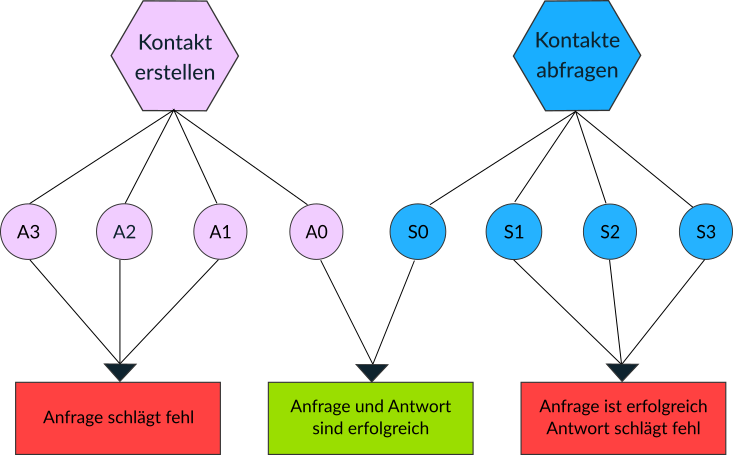
\includegraphics[width=0.8\textwidth]{Szenarien}
  \grayRule
  \caption{Szenarien bei der Datenübertragung über das Netzwerk}
  \label{fig:szenarien}
\end{figure}

%
% ERGEBNIS
%
\subsubsection*{Ergebnis}
Da die Szenarien \it{C0} und \it{S0}, \it{C1} und \it{C2} sowie \it{S1}, \it{S2} und \it{S3} zusammengefasst werden können, ergeben sich aus den sieben Szenarien die drei nun aufgezählten Fälle.
\begin{itemize}
  \item Fall a: Anfrage und Antwort sind erfolgreich.
  \item Fall b: Anfrage ist nicht erfolgreich
  \item Fall c: Anfrage ist erfolgreich, Antwort schlägt fehl
\end{itemize}
Von den erarbeiteten Fällen sind Fall \it{b} und \it{c} für die Szenarien zur Konfliktentstehung relevant.
% Die Anfrage schlägt fehl und die Anfrage ist erfolgreich aber die Antwort schlägt fehl.
%
%
% Konflikte-------------------------------------------------------------
%
\section{\label{chap:konfliktszenarien}Szenarien zur Konfliktentstehung}
Im Anwendungsbeispiel einer kollaborativen Kontaktliste können mehrere Personen die Liste verwalten. Oder eine Person benutzt die Anwendung auf mehreren Geräten, was zum selben Ergebnis führt:
Die Komplexität wird durch mehr Parteien -- beliebig viele Clients -- erhöht.
Jede Person kann alle Einträge jederzeit laden und einzelne erstellen, bearbeiten oder löschen. Bei den Ausführungen der grundlegenden \gls{CRUD}--Operationen, kann es bei der Synchronisation der beteiligten Parteien zu Konflikten kommen wenn einer der oben genannten Fälle \it{b} oder \it{c} eintritt und ein Objekt von mehreren Parteien bearbeitet wird.\\\\
Laut den Aussagen von Jan Lenhardt\footnote{ Mitgründer und Geschäftsführer der Neighbourhoodie Software GmbH, Committer und Vice President von Apache CouchDB}, die er in einem Interview getroffen hat, ergeben sich unterschiedliche, angewandte Vorgehensweisen, Objekte für die Verwendung in verteilten Systemen zu identifizieren und versionieren.
Nachfolgend werden diese Vorgehensweisen berücksichtigend, Konfliktszenarien dargestellt.
Es ist zu erwähnen, dass es bei diesen Methoden nicht immer zu Konflikten kommen muss.
Da es Thema dieser Arbeit ist, wird für jede Variante nur der ungünstigste Fall, der Konfliktfall beschrieben.
% \note{Damit die Einträge sortiert und gefiltert aus der Datenbank geladen werden können, werden sie mit einem Index versehen. Jeder neue Eintrag bekommt automatisch einen höheren Index. Die aktualisierten Objekte sollen ebenfalls geladen werden, aber keinen neuen Index bekommen. Deswegen gibt es neben dem Datensatz \sc{Adressbucheinträge} zusätzlich den der \sc{Aktualisierungen} mit einem sich automatisch erhöhendem Index \it{und der Referenz zum Adressbucheintrag}. \todo{eigenes Szenario?}. Mit jeder Aktualisierung oder Löschung eines Kontakts wird im Aktualisierungsdatensatz der Index durch einen neuen ersetzt. So hat jede Kontakt-ID eine Aktualisierungs-ID und ein Eintrag wird auch nach mehrmaligem Aktualisieren nicht mehrfach geladen.}\\
%
%
% Footnotes
%
\def \naturalkey {Ein Schlüssel, der sich aus einem Attribut des Objekts ergibt oder sich aus mehreren Attributen zusammensetzt. So könnte ein sprechender Schlüssel von Jean-Luc Picard mit der E-Mail-Adresse picard@enterpise.com beispielsweise `picard@enterprise.com` (E-Mail) oder `Jean-LucPicard` (Zusammensetzung aus Vor- und Nachnamen) sein.}
\def \logicalclock {Eine Logische Uhr ist eine Komponente die dazu dient, dem Datenobjekt einen eindeutigen Zeitstempel zuzuweisen. Die bekanntesten Verfahren für Logische Uhren in verteilten Systemen sind die Lamport-Uhr und die Vektoruhr. Beide verwenden Zähler die sich bei jedem Ereignis erhöhen. Einfach gesagt besteht die Lamport-Uhr aus einem Zeitstempel und einem Zähler, die Vektoruhr aus einem Zeitstempel und einem Vektor -- einer Liste aus Zählern.}
%
%
\begin{description}[leftmargin=0.5cm,style=nextline]
  % ID
  \item[Szenario ID0 -- UUID:]
    Zur Identifizierung eines Adressbucheintrags wird eine \gls{UUID} verwendet. Es wird sowohl auf dem Client als auch auf dem Server ein Kontakt mit dem Namen `Amilia Pond` erstellt.
    Währenddessen tritt Fall \it{b} oder \it{c} ein und beide Parteien können nicht miteinander kommunizieren. Nach der Synchronisation existieren zwei Kontakteinträge mit gleichem Namen, aber unterschiedlicher ID.
    Sie sind voneinander zu unterscheiden und können einzeln behandelt werden.\\
  \item[Szenario ID1 -- sprechender Schlüssel:]
    Zur Identifizierung eines Adressbucheintrags wird ein sprechender Schlüssel\footnote{\naturalkey} verwendet.
    Es wird sowohl auf dem Client als auch auf dem Server ein Kontakt mit dem Namen `Amilia Pond` und dem sprechenden Schlüssel `amiliapond` erstellt. Währenddessen tritt Fall \it{b} oder \it{c} ein.
    Es ist nicht zu ermitteln, ob derselbe Kontakt doppelt angelegt wurde, wenn beide Kontakteinträge sich unterscheiden, welcher der beiden korrekt ist oder ob es sich bei den Einträgen um zwei Personen mit demselben Namen handelt.\\
  %
  %
  % Version
  \item[Szenario V0 -- Versionsnummer:]
    Zur Versionierung eines Adressbucheintrags werden Versionsnummern verwendet. Der Kontakt `Amilia` hat die Version `1.0.0`.
    Sowohl auf dem Client, als auch auf dem Server wird der Kontakt bearbeitet und aktualisiert und geben ihm beide die Versonsnummer `2.0.0`.
    Währenddessen tritt Fall \it{b} oder \it{c} ein und beide Parteien können nicht miteinander Kommunizieren.
    Bei der Synchronisation entsteht ein Konflikt weil es zwei unterschiedliche Einträge mit derselben Verion gibt.\\
  %
  % Zeitstempel
  \item[Szenario V1  -- Zeitstempel:]
    Zur Versionierung eines Adressbucheintrags wird ein Zeitstempel verwendet. Der Kontakt `Amilia` hat die initiale Version `2018-04-03 10:00:00Z`.
    Amilia ist umgezogen und ihre Adresse ändert sich. Der Eintrag wird bearbeitet und hat nun die Version `2018-04-13 11:44:22Z`.
    Während der Editierung tritt Fall \it{b} oder \it{c} ein.
    Es stellt sich heraus, dass die Hausnummer einen Zahlendreher hat und es wird sofort, immernoch offline, berichtigt. `Amilia` hat nun die Version `2018-04-13 11:45:33Z`.\\
    Der Server hat eine eigene Uhr mit spätere Uhrzeit als der Client.
    So hat nach der Synchronisation der später korrigierte Eintrag einen früheren Zeitstempel.
    Es wird die falsche, alte Adresse gespeichert, die korrekte hat den älteren Zeitstempel und wird verworfen.\\
    Diese Variante funktioniert in vielen Fällen gut. Trotzdem kommt es selbst in großen Firmen wie Google zu Problemen\footnote{\url{https://support.google.com/accounts/answer/185834?hl=en\#sync}} wenn verschiedene Geräte eine eigene Uhr besitzen.\\
    Des Weiteren gibt es die Möglichkeit, dass auf dem einen Gerät die Hausnummer berichtigt wurde und auf einem anderen, zur ungefähr selben Zeit, ein Zusatz zur Adresse gespeichert wird. Das könnte die Etage sein in der Amilia wohnt. Dann gibt es zwei Versionen mit unterschiedlichen Zeitstempeln und eine davon wird in jedem Fall verworfen. Auch wenn beide Versionen richtig sind.\\
  %
  % Logische Uhr
  \item[Szenario V2 -- Logische Uhr:]
    Weil der Zeitstempel so fehleranfällig ist, wurde die Logische Uhr zur Versionierung von Objekten in Verteilten Systemen die Logische Uhr entwickelt.\\
    Zur Versionierung eines Adressbucheintrags wird eine Logische Uhr\footnote{\logicalclock} verwendet. Der Kontakt `Amilia` hat die Version \todo{Beispiel Logische Uhr?}.
    Amilias Adresse ändert sich und wird auf dem Client angepasst.
    Währenddessen tritt Fall \it{b} oder \it{c} ein.
    Amilia sieht ihre falsche Hausnummer und berichtigt diese ebenfalls.
    Bei der Synchronisation kommt es zum Konflikt. \todo{wirklich? auch wenn das Ergebnis dasselbe ist?}\\
    %
    % Hash
    % hash:  { name: Amilia Pond, phone: 0152397645, email: Amilia@pond.com }
  \item[Szenario V3 -- Inhaltsbasierte Version:]% CAV fail
    Zur Versionierung eines Adressbucheintrags wird eine inhaltsbasierte Version verwendet. Um eine Zuordnung zwischen Inhalt und Version machen zu können kommen \Glspl{Hashfunktion} zum Einsatz. Hierbei wird als Version der Hashwert des Adressbucheintrags gespeichert.\\
    Dem Kontakt `Amilia` ist die Version `5560348cec1b08c3d53e1508b4a46868` zugeordnet. Amilias Telefonnummer ändert sich und wird auf dem Client angepasst, während dieser offline ist.
    Im selben Status berichtigt der Client die Telefonnummer. Bei der Synchronisation kommt es zum Konflikt, da es nun zwei Einträge mit unterschiedlichem Inhalt, aber identischer Version gibt und nicht festzustellen ist welche Version die neuere ist.\\
    %
    % Hash Liste
  \item[Szenario V4 -- Liste von inhaltsbasierten Versionen:]
    Zur Versionierung eines Adressbucheintrags wird eine geordnete Liste von inhaltsbasierten Versionen verwendet.
    Dem Kontakt `Amilia` ist eine Liste von Verionen mit einem Eintrag `5560348cec1b08c3d53e1508b4a46868` zugeordnet.
    Amilias Telefonnummer ändert sich und wird auf dem Client angepasst, während dieser offline ist. Im selben Status berichtigt der Client die Telefonnummer.
    Jede Aktion fügt der Versionsliste einen neuen Hashwert hinzu.
    Auch wenn der Content des Adressbucheintrags in den zwei letzten Versionen identisch ist, kann festgestellt werden welcher der neueste Eintrag ist.
    Bei der Synchronisation kommt es zum Konflikt weil der Kontakt Amilia mit unteschiedlichen Informationen existiert.\\
    Beide konfliktbehafteten Versionen werden verschachtelt in der Liste gespeichert.
    In diesem Fall sieht die Liste nun so aus: `[[88da3f8d82ab58551d2a48d74d9a4986, 88da3f8d82ab58551d2a48d74d9a4986], 5560348cec1b08c3d53e1508b4a46868]` -- eine Liste der beiden konfliktbehafteten Versionen am Anfang der Liste.
\end{description}
% \begin{figure}[H]
%   \centering
%   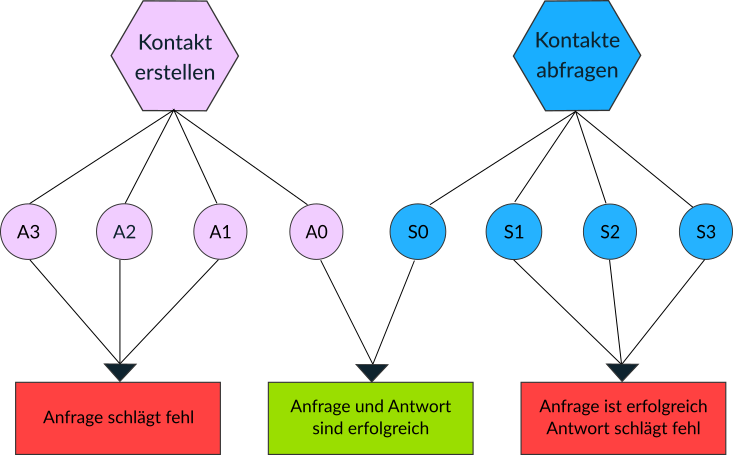
\includegraphics[width=0.8\textwidth]{Szenarien}
%   \grayRule
%   \caption[Szenarien]{Szenarien und Fälle}
%   \label{fig:scenarios}
% \end{figure}
%
% ERGEBNIS
%
\subsubsection*{Ergebnis}
Die Szenarien \it{ID0} und \it{ID1} beschreiben die Identifizierung einzelner Kontakte. Eine eindeutige Identifizierung des Kontakts ist im Szenario \it{ID0}, mittels der Verwendung einer \gls{UUID}, gewährleistet.\\
% Die Szenarien \it{V1}, \it{V2} und \it{V4}, \it{V5} beschreiben Situationen mit demselben Ausgangspunkt. In einem Fall kommt zu keinem Konflikt, in dem nächsten schon. Deswegen können \it{V1} und \it{V2}, sowie \it{V4} und \it{V5} zusammengefasst werden.
Es wird deutlich, dass es in jedem Fall zu einem Konflikt kommen kann. Es gilt zu unterscheiden in welchen Fällen mit Konflikten umgegangen werden muss weil sonst Daten verloren gehen.
\\\\
Im weiteren Verlauf dieser Arbeit werden aus dieser Erkenntnis die Anforderungen an eine offlinefähige Anwendung erarbeitet.